\section{Repr�sentation von Suchr�umen}

\subsection{Suchraum als Karte}

Ein Suchraum wird normalerweise als grafische Karte dargestellt. Diese Karten k�nnen als Wegenetz oder als Gitter mit benachbarten Zellen dargestellt werden, wie in Abbildung \ref{fig:graph-examples} gezeigt.

\begin{figure}[H]
    \centering
    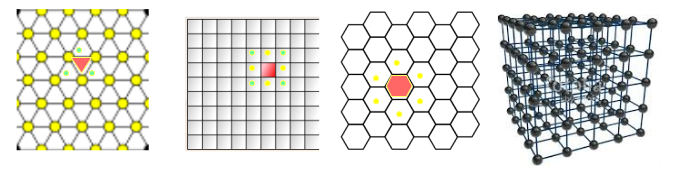
\includegraphics[width=\textwidth]{figures/kap3/graph-examples.png}
    \caption{Beispiele von Gittermustern}
    \label{fig:graph-examples}
\end{figure}

Je nach verwendetem Gittermuster werden unterschiedliche Suchgraphen basierend auf der Anzahl der Nachbarn jeder Zelle im Gitter gebildet. Zum Beispiel: Eine dreieckige Zelle hat sechs Nachbarn, eine quadratische Zelle hat 4 (oder 8, wenn Diagonalen erlaubt sind) und eine sechseckige Zelle hat 6.